\apendice{Plan de Proyecto Software}

\section{Introducción}

En este apartado se procederá a explicar con detalle cual ha sido el resultado de la planificación del proyecto.

Está planificación se ha realizado utilizando  una metodología ágil basada en \emph{sprints} de una duración de una o dos semanas en función de las necesidades y el tiempo disponible debido a otras cargas de trabajo diferentes a este proyecto.

En estos \emph{sprints} se van marcando ciertos objetivos que serán revisados junto a los tutores en las reuniones al final de los mismos. Los objetivos del siguiente \emph{sprint} serán marcados durante dichas reuniones.
 
Para el control de tiempos se ha utilizado la herramienta ZenHub siendo la valoración de los \emph{Story Points} la siguiente:

\begin{comment}
\begin{table}[]
\begin{center}
\begin{tabular}{|l|l|}
\hline
Story Points & Estimación temporal \\ \hline
1            & 30 min              \\ \hline
2            & 1 hora              \\ \hline
3            & 1,5 horas           \\ \hline
4            & 2 horas             \\ \hline
5            & 2,5 horas           \\ \hline
6            & 3 horas             \\ \hline
7            & 3,5 horas           \\ \hline
8            & 4 horas             \\ \hline
9            & 6 horas             \\ \hline
10           & 8 horas             \\ \hline
\end{tabular}
\caption{Equivalencias \emph{Story Points} y tiempo estimado}
\label{tabla:StoryPoints/tiempo}
\end{center}
\end{table}
\end{comment}

Aclarar que los gráficos \emph{Burn Down} de los primeros \emph{sprints} no están todo lo bien que deberían por la poca experiencia con la herramienta.

\textcolor{red}{cambio valor story points aqui o en sprint ¿?}
 
\textcolor{red}{etiquetas}

\section{Planificación temporal}

\subsection{Sprint 1(29/01/2020 - 05/02/2020)}\label{Sprint-1}
En esta primera reunión se marcó el comienzo del proyecto. Ya se había hablado anteriormente con uno de los tutores (Jose Francisco) del interés sobre el proyecto propuesto del que también formaba parte de los tutores Alvar Arnaiz.

Al ser la primera reunión se hablo de las herramientas que se iban a utilizar así como acordar los primeros objetivos de este \emph{sprint}:

\begin{itemize}
\item - Crear el repositorio.
\item - Añadir la plantilla de Latex a la documentación.
\item - Crear cuenta en la plataforma \emph{Copernicus}.
\item - Investigar el funcionamiento básico de las librerías a utilizar.
\item - Leer una serie de papers que me proporcionaron sobre las medusas.
\end{itemize}

Se estimó unas 10 horas de trabajo de las que finalmente se invirtieron 8 horas quedando sin terminar una \emph{issue}.

\begin{center}
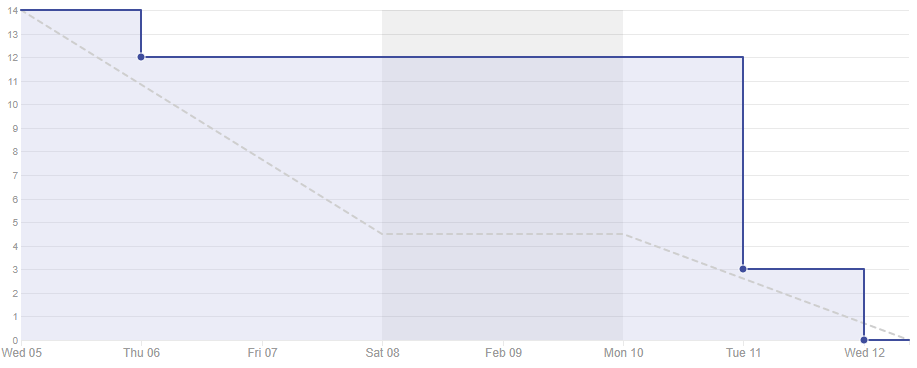
\includegraphics[scale=0.5]{Sprint1_BurnDown}
\end{center}

\section{Estudio de viabilidad}

\subsection{Viabilidad económica}

\subsection{Viabilidad legal}


